\documentclass{article} % For LaTeX2e
\usepackage{nips14submit_e,times}
\usepackage{hyperref}
\usepackage{url}
\usepackage[leqno, fleqn]{amsmath}
\usepackage{amssymb}
\usepackage{qtree}
\usepackage[numbers]{natbib}
\usepackage{graphicx}
\usepackage{booktabs}
\usepackage{colortbl}
\usepackage{caption}
\usepackage{subcaption}
\usepackage{xcolor}



\definecolor{mylinkcolor}{rgb}{0,0,0} % black
\hypersetup{colorlinks, linkcolor=mylinkcolor, urlcolor=mylinkcolor, citecolor=mylinkcolor}

\newcommand{\nateq}{\equiv}
\newcommand{\natind}{\mathbin{\#}}
%\newcommand{\natneg}{\raisebox{2px}{\tiny\thinspace$\wedge$\thinspace}}
\newcommand{\natneg}{\mathbin{^{\wedge}}}
\newcommand{\natfor}{\sqsubset}
\newcommand{\natrev}{\sqsupset}
\newcommand{\natalt}{\mathbin{|}}
\newcommand{\natcov}{\mathbin{\smallsmile}}

\newcommand{\plneg}{\mathop{\textit{not}}}
\newcommand{\pland}{\mathbin{\textit{and}}}
\newcommand{\plor}{\mathbin{\textit{or}}}



% Strikeout
\newlength{\howlong}\newcommand{\strikeout}[1]{\settowidth{\howlong}{#1}#1\unitlength0.5ex%
\begin{picture}(0,0)\put(0,1){\line(-1,0){\howlong\divide\unitlength}}\end{picture}}

\newcommand{\True}{\texttt{T}}
\newcommand{\False}{\texttt{F}}
\usepackage{stmaryrd}
\newcommand{\sem}[1]{\ensuremath{\llbracket#1\rrbracket}}


\renewcommand{\bibsection}{\subsubsection*{References}}

\usepackage{gb4e}

\def\ii#1{\textit{#1}}

\newcommand{\mynote}[1]{{\color{red}\framebox{\begin{tabular}{p{0.9\textwidth}}\footnotesize#1 \end{tabular}}}}


\title{Recursive Neural Networks for Learning Logical Semantics}

\author{
Samuel R.\ Bowman$^{\ast\dag}$ \\
\texttt{sbowman@stanford.edu} \\[2ex]
$^{\ast}$Stanford Linguistics \\
\And
Christopher Potts$^{\ast}$\\
\texttt{cgpotts@stanford.edu} \\[2ex]
$^{\dag}$Stanford NLP Group
\And
Christopher D.\ Manning$^{\ast\dag\ddag}$\\
\texttt{manning@stanford.edu}\\[2ex]
$^{\ddag}$Stanford Computer Science
}

% \author{
% Samuel R.\ Bowman \\
% NLP Group, Dept.\ of Linguistics\\
% Stanford University\\
% Stanford, CA 94305-2150 \\
% \texttt{sbowman@stanford.edu}
%  \And
%  Christopher Potts \\
% Dept.\ of Linguistics\\
% Stanford University\\
% Stanford, CA 94305-2150 \\
% \texttt{cgpotts@stanford.edu}
%  \And
% Christopher D.\ Manning \\
% NLP Group,  Depts.\ of Computer Science and Linguistics\\
% Stanford University\\
% Stanford, CA 94305-2150 \\
% \texttt{manning@stanford.edu}
% }

\newcommand{\fix}{\marginpar{FIX}}
\newcommand{\new}{\marginpar{NEW}}

\nipsfinalcopy % Uncomment for camera-ready version

\begin{document}
\maketitle

% Compare with Grefenstette etc?

  Supervised recursive neural network models (RNNs) for sentence
  meaning have been successful in an array of sophisticated language
  tasks, but it remains an open question whether they can learn
  compositional semantic grammars that support logical deduction.  We
  address this question directly by for the first time evaluating
  whether each of two classes of neural model --- plain RNNs and
  recursive neural tensor networks (RNTNs) --- can correctly learn
  labelships such as entailment and contradiction between pairs of
  sentences, where we have generated controlled data sets of sentences
  from a logical grammar.  Our first experiment evaluates whether
  these models can learn the basic algebra of logical labels
  involved. Our second and third experiments extend this evaluation to
  complex recursive structures and sentences involving quantification.
  We find that the plain RNN achieves only mixed results on all three
  experiments, whereas the stronger RNTN model generalizes well in
  every setting and appears capable of learning suitable
  representations for natural language logical inference.

\subsection*{Recursive neural network models}

\begin{figure}[hp]
  \centering\resizebox{4.5in}{!}{
  \begin{subfigure}[t]{0.45\textwidth}
\centering
\scalebox{0.75}{
 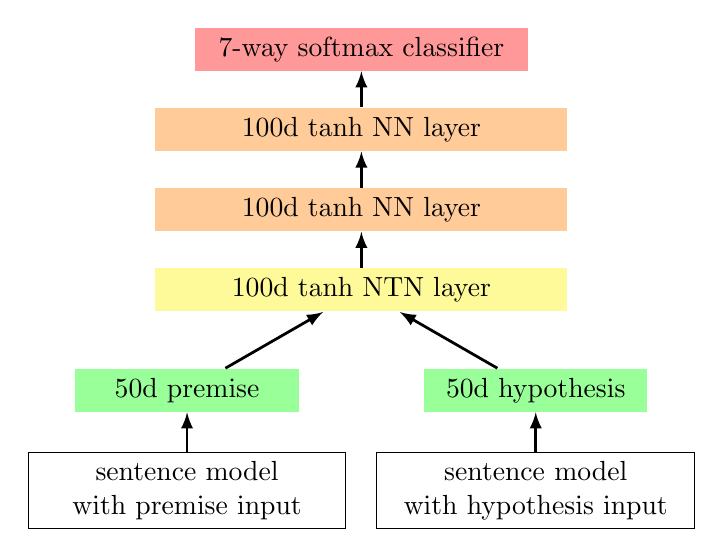
\begin{tikzpicture}
    \def\dx{21pt}
    \def\dy{29pt}

    \tikzstyle{label}=[text width=40mm,align=center]    
    \tikzstyle{softmax}=[fill=red!40,text width=40mm,align=center]
    \tikzstyle{preclass}=[fill=orange!40,text width=50mm,align=center]
    \tikzstyle{e}=[fill=green!40,text width=26mm,align=center]
    \tikzstyle{m}=[draw=black,text width=38mm,align=center]    
    
    \node[softmax]  (softmax) at (0*\dx,6*\dy) {7-way softmax classifier};
    \node[preclass]  (pc3) at (0*\dx,5*\dy) {100d $\tanh$ NN layer};
    \node[preclass]  (pc2) at (0*\dx,4*\dy) {100d $\tanh$ NN layer};
    \node[preclass,fill=yellow!40]  (pc1) at (0*\dx,3*\dy) {100d $\tanh$ NTN layer};
    \node[e]  (pe) at (-3*\dx,1.75*\dy) {50d premise};
    \node[e]  (he) at (3*\dx,1.75*\dy) {50d hypothesis};
    \node[m]  (pem) at (-3*\dx,0.5*\dy) {sentence model\\ with premise input};
    \node[m]  (hem) at (3*\dx,0.5*\dy) {sentence model\\ with hypothesis input};    
    
    \pgfsetarrowsend{latex}
    \tikzstyle{fwd} = [draw=black, line width=1pt]

          \draw [fwd] (pc3) -- (softmax);
          \draw [fwd] (pc2) -- (pc3);
          \draw [fwd] (pc1) -- (pc2);
          \draw [fwd] (pe) -- (pc1);
          \draw [fwd] (he) -- (pc1);
          \draw [fwd] (hem) -- (he);
          \draw [fwd] (pem) -- (pe);

  \end{tikzpicture}}
  
 \caption{The general architecture shared across models.}\label{fig:model:top}
  
\end{subfigure}

\begin{subfigure}[t]{0.45\textwidth}
  \centering
\scalebox{0.75}{
 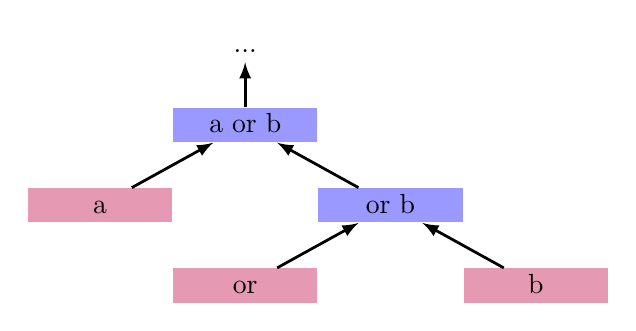
\begin{tikzpicture}
    \def\dx{21pt}
    \def\dy{29pt}


    \tikzstyle{word}=[fill=purple!40,text width=16mm,text height=2mm,align=center]
    \tikzstyle{node}=[fill=blue!40,text width=16mm,text height=2mm,align=center]
    \tikzstyle{empty}=[fill=blue!0,text width=8mm,text height=2mm,align=center]

    \node[empty]  (null) at (0*\dx,7*\dy) {...};
    \node[node]  (aorb) at (0*\dx,6*\dy) {a or b};
    \node[word]  (a) at (-2.5*\dx,5*\dy) {a};
    \node[node]  (orb) at (2.5*\dx,5*\dy) {or b};
    \node[word]  (or) at (0*\dx,4*\dy) {or};
    \node[word]  (b) at (5*\dx,4*\dy) {b};
    
    
    \pgfsetarrowsend{latex}
    \tikzstyle{fwd} = [draw=black, line width=1pt]

          \draw [fwd] (or) -- (orb);
          \draw [fwd] (b) -- (orb);
          \draw [fwd] (a) -- (aorb);
          \draw [fwd] (orb) -- (aorb);
          \draw [fwd] (aorb) -- (null);
  \end{tikzpicture}}
  
     \caption{The architecture for the TreeRNN and TreeRNTN sentence models. Terminal nodes are learned embeddings and nonterminal nodes are either NN or NTN layers with $\tanh$ nonlinearities.}\label{fig:model:tree}
  
  \end{subfigure}
 \vspace{0.5cm}
  
\begin{subfigure}[t]{0.45\textwidth}
  \centering
\scalebox{0.75}{
 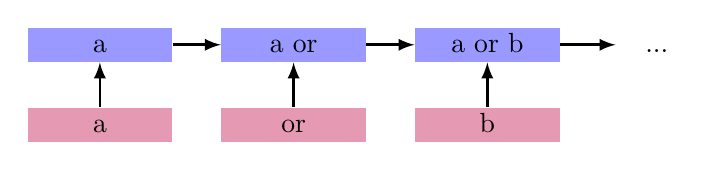
\begin{tikzpicture}
    \def\dx{35pt}
    \def\dy{29pt}


    \tikzstyle{word}=[fill=purple!40,text width=16mm,text height=2mm,align=center]
    \tikzstyle{node}=[fill=blue!40,text width=16mm,text height=2mm,align=center]
    \tikzstyle{empty}=[fill=blue!0,text width=8mm,text height=2mm,align=center]

    \node[word]  (a) at (-3*\dx,1*\dy) {a};
    \node[node]  (aN) at (-3*\dx,2*\dy) {a};
    
    \node[word]  (or) at (-1*\dx,1*\dy) {or};
    \node[node]  (orN) at (-1*\dx,2*\dy) {a or};
    
    \node[word]  (b) at (1*\dx,1*\dy) {b};
    \node[node]  (bN) at (1*\dx,2*\dy) {a or b}; 
    
    \node[empty]  (nullN) at (2.75*\dx,2*\dy) {...}; 
    
    \pgfsetarrowsend{latex}
    \tikzstyle{fwd} = [draw=black, line width=1pt]

          \draw [fwd] (or) -- (orN);
          \draw [fwd] (b) -- (bN);
          \draw [fwd] (a) -- (aN);
          \draw [fwd] (aN) -- (orN);
          \draw [fwd] (orN) -- (bN);
          \draw [fwd] (bN) -- (nullN);
          
  \end{tikzpicture}}
  
   \caption{The architecture for the LSTM sentence model. Nodes in the lower row are learned embeddings and nodes on the upper row are LSTM units.}\label{fig:model:seq}
  
    \end{subfigure}}
  % \caption{The model structure used to compare \ii{((all reptiles) walk)} and \ii{((some turtles) move)}. 
  %  The same structure is used for both the RNN and RNTN layer functions.} 
  \label{sample-figure}
\end{figure}

In our experiments, we train pairs of recursive (tree structured) neural network models \cite{socher2013acl1} which are joined together with a shared top layer that generates features for a classifier. The classifier predicts the logical label that holds between the sentences represented by the two trees (entailment in the above; the table below reviews the full inventory of labels we predict). For an activation function, we use either a plain NN layer or a tensor combination layer.

% TODO gold parse structures

\subsection*{Inference and the semantic labels}

Our aim is to evaluate the ability of learned recusive models to represent semantic structure. We pursue this through an inference task, where the models must learn to choose the logical label that applies between a pair of statements. The possible labels are the seven below from \cite{maccartney2009extended}. This is distinct from the limited prior work on learning neural network models for formal semantics \cite{grefenstette2013towards, rocktaschellow}, which use an interpretation task in which the model evaluates sentences as \textit{true} or \textit{false} with respect to some representation of the world. Our approach allows us to sidestep serious open problems involved in the representation of a complete set of knowledge about the world.

\begin{table}[h]\small
\centering\resizebox{4.5in}{!}{
  \setlength{\tabcolsep}{15pt}
  \renewcommand{\arraystretch}{1.1}
  \begin{tabular}{l c l l} 
    \toprule
    Name & Symbol & Set-theoretic definition & Example \\ 
    \midrule
    entailment         & $x \natfor y$   & $x \subset y$ & \ii{turtle, reptile}  \\ 
    reverse entailment & $x \natrev y$   & $x \supset y$ & \ii{reptile, turtle}  \\ 
    equivalence        & $x \nateq y$    & $x = y$       & \ii{couch, sofa} \\ 
    alternation        & $x \natalt y$   & $x \cap y = \emptyset \wedge x \cup y \neq \mathcal{D}$ & \ii{turtle, warthog} \\ 
    negation           & $x \natneg y$   & $x \cap y = \emptyset \wedge x \cup y = \mathcal{D}$    & \ii{able, unable} \\
    cover              & $x \natcov y$   & $x \cap y \neq \emptyset \wedge x \cup y = \mathcal{D}$ & \ii{animal, non-turtle} \\ 
    independence       & $x \natind y$   & (else) & \ii{turtle, pet}\\
    \bottomrule
  \end{tabular}}
  \label{b-table}
\end{table}

\subsection*{Reasoning with atomic symbols}

If any model is to learn the behavior of a labelal logic like the one presented here from a finite amount of data, it must learn to deduce new labels from already seen labels. Our first experiment evaluates the ability of our models to do this over pairs of atomic symbols. The model is trained on a randomly generated set of consistent statements like \{$a \natfor b$, $b \natfor c$, $c \natneg d$\}, and tested on novel examples that follow from the statements seen in training, like \{$a \natfor c$\}. A tuned RNTN reached greater than 99\% test accuracy, but no plain RNN surpassed 89\%.

\subsection*{Recursive structure in propositional logic}\label{sec:recursion}

Our second experiment introduces compositional structure to our examples, replacing the atomic statements above with pairs of short statements of propositional logic, like $\plneg a\natalt((a~(\pland~ b))~(\pland~c))$. We train our models on only pairs of statements with up to four symbols (corresponding to test accuracy figures to the left of the dashed line below), but observe that the RNTN performs reasonably both on pairs of that length and on much longer test pairs. 

\begin{figure}[h]
  \centering
  \includegraphics[width=4in]{recursion\string_results\string_final.eps}
  \label{prop-results}
\end{figure} \vspace{-.3cm}

\subsection*{Reasoning with natural language quantifiers and negation}\label{sec:quantifiers}

For our third experiment, we generate pairs of sentences in which each sentence contains one quantifier, and any of a small set of common nouns, as in the example \textit{(no warthogs) move $\natfor$ (no (not reptiles)) swim}. The parentheses indicate the tree structure for each sentence as it will be used by the model. We defined several different types of train--test split for this experiment. RNTNs performed either well ($>85\%$ accuracy) or perfectly on all of them, while plain RNNs did not break 80\% in any setting. These experiments differentiate the increased power of RNTNs better than previous work and provide the most convincing demonstration to date of the ability of neural networks to model semantic inferences in complex natural language sentences.


\bibliographystyle{unsrtnat}

\small % Note: Explicitly allowed in style guide
\bibliography{MLSemantics} 

\end{document}
